\pdfinfo{
/ModDate (\pdfcreationdate)                                   
/Producer (pdfLaTeX)                                    
}


\documentclass[fleqn,oneside,openany,a4paper,11pt]{book}

\usepackage{color}
\usepackage[utf8]{inputenc}
\usepackage[breaklinks]{hyperref} %
\usepackage{pracadok}
\usepackage{longtable}
%\usepackage{array}
%\usepackage{geometry}
%\usepackage{fancyhdr}
\usepackage{float}

\pdfcompresslevel=9

\def\uwaga#1{}

\begin{document}
\let\s\lstinline
\lstset{inputencoding=utf8, extendedchars=true,literate={ą}{{\k{a}}}1 {ć}{{\'c}}1 {ę}{{\k{e}}}1 {ł}{{\l{}}}1 {ń}{{\'n}}1 {ó}{{\'o}}1 {ś}{{\'s}}1 {ż}{{\.z}}1 {ź}{{\'z}}1 {Ą}{{\k{A}}}1 {Ć}{{\'C}}1 {Ę}{{\k{E}}}1 {Ł}{{\L{}}}1 {Ń}{{\'N}}1 {Ó}{{\'O}}1 {Ś}{{\'S}}1 {Ż}{{\.Z}}1 {Ź}{{\'Z}}1}

% Tytuł
\def\autor{Informatyka Stosowana III rok}
\def\tytul{\textbf{\LARGE Zespołowe Przedsięwzięcie Inżynierskie}}
\def\promotor{~}
\def\miejscerokwydania{Nowy Sącz \today}
\def\nazwauczelni{PAŃSTWOWA WYŻSZA SZKOŁA ZAWODOWA}
\def\imienia{INSTYTUT  TECHNICZNY}
\def\wydzial{Kierunek Informatyka Stosowana}

\thispagestyle{empty}
{
\hbox{}\vskip 0.3\textheight
\hspace{1cm}
\centering
\vbox{
\noindent\textbf{\Huge Regulamin \\ \vspace{0.3cm}turnieju szachowego}\vspace{0.5cm}\\
}
\definecolor{tlo}{rgb}{.7,.7,.7} 
\lstset{language=bash,commentstyle=\scriptsize,backgroundcolor=\color{tlo},%
basicstyle=\scriptsize}

%spis tresci
{\footnotesize\tableofcontents}

\setcounter{chapter}{0}
%Opis wykonywanego zadania
%Cel
%Zakres prac
%Interesariusze
\chapter{Zespołowe przedsięwzięcie}

\begin{itemize}
\item Zespołowe przedsięwzięcie inżynierskie oznaczać będzie projekt, działanie podjęte w realizacji postawionego celu, realizowane zespołowo.
\item Projekt jest odpowiedzią na problem/potrzebę, w określonej przestrzeni życia.
\end{itemize}

\section{Członkowie zespołu z określeniem funkcji}
\begin{description}
\item[1] Piotr Jabloński - programista Java
\item[2] Mirosława Pelc - programista Java
\item[3] Mariusz Lorek - kierownik zespołu, testowanie, przygotowanie dokumentacji
\end{description}

\section{Uzasadnienie potrzeby realizacji projektu}
Potrzebny jest program który wspomoże zorganizowanie turnieju szachowego w którym może wziąść udział dowolna, nieznana wcześniej liczba zawodników. Czas trwania turnieju jest ograniczony przez organizatora. Turniej szachowy jest organizowany cyklicznie, dlatego stworzenie programu wspomagającego jego obsługę znacznie ułatwi przeprowadzanie kolejnych edycji.


\section{Cele projektu}
\begin{enumerate}
\item Stworzenie programu wspomagającego organizację turnieju szachowego.
Napisany program ma pozwolić na sprawne przeprowadzenie turnieju szachowego i wyłonienie zwycięzcy turnieju i/lub zawodników którzy zajeli kolejne miejsca w turnieju.
\item Przygotowanie instrukcji obsługi programu/aplikacji dla użytkownika końcowego
\end{enumerate}
 


\section{Zakres projektu}
\begin{enumerate}
	\item Stworzenie programu do wspomagania organiacji turnieju szachowego według wytycznych zleceniodawcy
	\item Stworzenie dokumentacji opisującej postępy prac nad tworzonym projektem z podziałem na czynności które ma wykonywać każdy z członków zespołu
\end{enumerate}
Gotowy program ma pozwalać m.in na:
\begin{itemize}
	\item Przeprowadzenie turnieju szachowego w systemie kołowym (każdy z każdym) z podziałem na grupy
	\item Zarzadzanie turniejami w bazie danych 
	\item Zgromadzenie podstawowych danych o zawodnikach, jakim są: (Imię, Nazwisko, Wiek, Kategoria szachowa) 
	\item Dodawanie, usuwanie i edycja zawodników, 
	\item Podział zawodników na grupy w ze względu na przedział wiekowy, kategorie szachową lub manualnie. 
	\item Ustalenie liczby grup oraz szachownic przed rozpoczęciem nowego turnieju. 
	\item Ustalanie uczestników każdego meczu - kolor pionków (biały, czarny) przydzielany do zawodników przed każdym spotkaniem 
	\item Punktowanie rozegranych spotkań
\end{itemize}


\section{Grupy docelowe}
Program przeznaczony dla organizatorów turniejów szachowych.  


\section{Struktura podziału prac (zadań) - WBS}

Program wspomagający przeprowadzenie turneju szachowego
\begin{enumerate}
\item Zebranie informacji na temat sposobu przprowadzania turnieju szachowego od zleceniodawcy
\begin{enumerate}
	\item Wybranie systemu według którego będzie przeprowadzany turniej, wybór najoptymalniejszego rozwiązania
	\item Przygotowanie regulaminu turnieju.
\end{enumerate}
\item Projekt programu
\begin{enumerate}
\item Określenie jakie elementy muszą się znaleść w programie
\item Szablon programu
\item Wybór narzędzi/aplikacji służących do napisania programu
\item Rozdzielenie zadań dla programistów
\end{enumerate}
\item Tworzenie programu/aplikacji
\begin{itemize}
\item Opracowanie narzędzi bazodanowych przechowujących informacje dotyczące turniejów
\item Przygotowanie elementów środowiska graficznego
\item Integracja narzędzi bazodanowych z elementami środowiska graficznego

\item Wstępna wersja programu
\item Testowanie
\begin{enumerate}
	\item Weryfikacja - "Czy budujemy prawidłowo produkt", dynamiczna i statyczna
	\item Walidacja - "Czy budujemy prawidłowy produkt"
	\item Testy
	\begin{itemize}
		\item Testy jednostkowe
		\item Testy integracyjne
		\item Testy systemowe
		\item Testy użyteczności
		\item Testy akceptacyjne (przeprowadzane przez zleceniodawce projektu
	)
	Testy mają za zadanie sprawdzenie każdego komponentu niezależnie
	\end{itemize}
\end{enumerate}
\item Eliminacja znalezionych błędów
\item Dodawanie kolejnych funkcji do programu

\end{itemize}
\item Końcowa wersja programu

\end{enumerate}

\section{Regulamin turnieju}
\begin{enumerate}
\item Obowiązują przepisy gry międzynarodowej federacji szachowej (fide).
\item Każdy z zawodników powinien się kierować zasadami fair play.
\item Zasady rozgrywki:
\begin{enumerate}
\item Turniej rozgrywany jest w dwóch fazach: grupowej i finałowej.\\
\item Tworzona jest lista startowa według przyjętych przez prowadzącego turniej kryteriów, domyślnie:
\begin{enumerate}
\item kategoria szachowa 
\item wiek
\item alfabetycznie
\end{enumerate}
\item Ilość grup jest zależna od liczby uczestników i ustala ją prowadzący.
\item Lista startowa dzielona jest na liczbę części równą liczbie grup
\item Następnie zawodnicy z każdej części są losowo rozmieszczani w grupach
\item W fazie grupowej prowadzone są rozgrywki, gdzie każdy gra z każdym w danej grupie.
\item W fazie finałowej zawodnicy wyłonieni z grup (liczbę osób wychodzących z grup ustala prowadzący) grają między sobą.
\item Turniej trwa maksymalnie 2.5 godziny z tego:
\begin{itemize}
\item 10 minut na przyjmowanie zgłoszeń(rejestrację),
\item 10 minut na losowanie spotkań,
\item Na każdą rozgrywaną partię przypada 10 minut. Każdy zawodnik ma 5 minut na wykonanie swoich posunięć.
\end{itemize}
\item Zawodnicy mają do dyspozycji zegar analogowy lub cyfrowy z 2 tarczami lub wyświetlaczami umożliwiający odmierzanie czasu rozgrywki dla każdego z zawodników osobno
\item Za zajecie ustalonych przez prowadzącego miejsc w turnieju zawodnicy otrzymują nagrody przewidziane przez organizatora.
\item Jeśli prowadzący ustali, uczestnicy będą mieli obowiązek zapisywać swoje ruchy na wydzielonych do tego kartkach.
\item Każdy stanowisko do gry ma swój numer identyfikacyjny, który obowiązuje przy rozgrywkach.
\item W sali, w której obywa się turniej szachowy zawodnicy jak i widzowie muszą zachować bezwzględną ciszę, aby nie przeszkadzać graczom w rozgrywce.
\item Jeśli jakiś uczestnik turnieju lub widz będzie podpowiadał innemu uczestnikowi, zawodnik otrzymuje od prowadzącego ostrzeżenie, w wypadku powtórzenia się sytuacji gracz któremu pomoc została ponownie udzielona może zostać zdyskwalifikowany z dalszych rozgrywek przez prowadzącego.
\item W turnieju obowiązuje punktacja
\begin{itemize}
	\item Za zwycięstwo - 1pkt
	\item Za remis - 0,5pkt
	\item Za porażkę - 0pkt
	\item Punkty pomocnicze, wykorzystywane gdy kilku zawodników ma taką samą liczbę punktów głównych, przyznawane po zakończeniu etapu (eliminacji lub finału) według schematu:
	\begin{itemize}
		\item Za zwycięstwo - punkty zawodników z którym dany zawodnik wygrał
		\item Za remis - połowę punktów zawodników z którym dany zawodnik zremisował
		\item Za porażkę - Nie są przyznawane punkty pomocnicze
	\end{itemize}
	\end{itemize}
\end{enumerate}
\item W razie rezygnacji lub wykluczenia zawodnika z turnieju, rozgrywki, które zagrał nie zostają anulowane, a osoby, które się z nim spotykają w dalszych rozgrywkach wygrywają walkowerem otrzymują 1pkt za zwycięstwo
\item W Sali zostało wydzielone pięć części:
\begin{enumerate}
\item Pierwsza, w której znajdują się tylko i wyłącznie osoby rozgrywające mecz
\item Druga, w której znajdują się widzowie bądź gracze, którzy obecnie nie rozgrywają żadnego spotkania
\item Trzecia, w której znajdują się stanowiska do gry w szachy poza turniejem
\item Czwarta, w której znajdują się gracze oczekujący na mecz
\item Piąta, w której znajduje się tylko i wyłącznie prowadzący turniej szachowy bądź osoby, które za zezwoleniem mogą znajdować się w tej strefie
\end{enumerate}
\item Zawodnicy, którzy nie grają lub czekają na swoją kolej w obrębie sali lub w niedalekiej odległości od niej w wypadku wezwania do rozgrywki powinni w trybie natychmiastowym zgłosić się do udziału w spotkaniu. W wypadku niestawienia się do rozegrania meczu zawodnik zostaję zdyskwalifikowany.
\item W przypadku, gdy:
\begin{itemize}
\item Zawodnik utrudnia przeprowadzanie rozgrywek może zostać zdyskwalifikowany z turnieju lub wyproszony z sali przez Prowadzącego.
\item Widz utrudnia przeprowadzanie rozgrywek może zostać wyproszony z sali przez Prowadzącego.
\end{itemize}
\item Udział w turnieju szachowym jest równoznaczny z zaakceptowaniem regulaminu
\end{enumerate}
%\section{Diagram sieciowy}
%Diagram sieciowy ukazuje zależności czasowe, węzły (aktywności), krawędzie (zależności czasowe).


\section{Harmonogram}
\subsection{Harmonogram prac poszczególnych członków zespołu}
\textbf{Mirosława Pelc oraz Piotr Jabłoński wspólna praca programistyczna\\
Mirosława Pelc - Odpowiedzialna w głównej mierze za interfejs graficzny\\
Piotr Jabłoński - Programowanie, algorytmy\\}
\begin{tabular}{|p{9cm}|l|p{3cm}|} \hline
Zadanie & Data rozpoczecia & Data zakończenia\\ \hline
Przygotowanie klas odpowiadających za uczestnika, turniej, rozgrywkęzygotowanie klas odpowiadających za uczestnika, turniej, rozgrywkę & 6.10.2015 & 20.10.2015 \\ \hline
Wyszukikawanie możliwych do wykorzystania elementów dostępnych w bibliotekach graficznych dla języka JAVA& 6.10.2015 & 20.10.2015 - zadanie ciągłe wykonywane przez cały czas trwania projektu\\ \hline
Integracja z bazą danych SQLite do przechowywania uczestników& &\\
Integracja z bazą danych SQLite do przechowywania turniejów&20.10.2015&27.10.2015\\
Integracja z bazą danych SQLite do przechowywania wyników pojedynczych rozgrywek&&\\ \hline
tabela - lista uczestników&27.10.2015&3.11.2015\\ \hline
dodawanie nowego uczestnika&27.10.2015&3.11.2015\\ \hline
usuwanie uczestnika&3.11.2015&10.11.2015\\ \hline
edycja uczestnika&3.11.2015&10.11.2015\\ \hline
dodawanie losowego uczestnika&10.11.2015&17.11.2015\\ \hline
symulacja ilości rozgrywek dla danej liczby uczestników, typu turnieju (systemem szwajcarskim / eliminacje grup)&10.11.2015&17.11.2015\\ \hline
podział graczy na grupy wg listy sortowanej po ustalanych przez prowadzącego turniej (dynamicznie w programie) warunkach takich, jak: kategoria zawodnika, wiek, nazwisko, imię lub przydział manualny&17.11.2015&24.11.2015\\ \hline
tworzenie początkowej listy graczy (sortowanie) do turnieju rozgrywanego systemem szwajcarskim (sortowanie po kategorii, wieku, nazwisko, imię)&17.11.2015&24.11.2015\\ \hline
dobieranie zawodników w pary dla systemu kołowego z eliminacjami w grupach - eliminacje
wybór zawodników przechodzących do finałów w rozgrywkach z eliminacjami
dobieranie zawodników w pary dla systemu kołowego z eliminacjami w grupach - finały&24.11.2015&1.12.2015\\ \hline
dobór zawodników w systemie kołowym (4 tyg!)&&\\ \hline 
lista wyników dla turnieju rozgrywanego systemem kołowym z eliminacjami&1.12.2015&8.12.2015\\ \hline
lista wyników dla turnieju rozgrywanego systemem szwajcarskim&&\\ \hline 
zastosowanie programu do prowadzednia kilku turniejów jednocześnie&&\\ \hline
usprawnienia ergonomii interfejsu&&praca ciągła do końca trwania projektu\\ \hline
usprawnienia estetyczne interfejsu&&praca ciągła do końca trwania projektu\\ \hline

\end{tabular}

\begin{tabular}{|p{9cm}|l|p{3cm}|} \hline
Zadanie & Data rozpoczecia & Data zakończenia\\ \hline
Przygotowanie dokumentacji dla projektu&&cały czas trwania projektu\\ \hline
Rozmowa ze zleceniodawcą na temat projektu &&20.10.2015\\ \hline
Wybór systemu w którym przeprowadzany będzie turniej &&27.10.2015\\ \hline
Okreslenie regulaminu turnieju (czas trwania,  system rozgrywego, określenie zasad uczestnictwa w turnieju, powody do dyskwalifikacji) &&3.11.2015\\ \hline
Opis repozytorium GitHub wykorzystywanego do pracy w projekcie &&17.11.2015\\ \hline
Przygotowywanie kolejnych części dokumentacji na podstawie informacji dostarczonych przez pozostałych członków zespołu&&\\ \hline
Testowanie kolejnych wersji  programu, wyszukiwanie błędów sugestie na temat usprawnień - praca ciągła, do końca trwania projektu&&\\ \hline
Konsultację ze zleceniodawcą na temat ewentualnych poprawek, dodawania nowych funkcjonalności wymaganych przez zleceniodawcę.&&\\ \hline 
\end{tabular}

\section{Dokumentacja}
Przygotowanie środowiska do równoległego opracowania dokumentacji projektu i realizacji przydzielonych zadań poszczególnym członkom zespołu projektowego.

\subsection[Edycja plików dokumentacyjnych]{Edycja plików dokumentacyjnych - każdy członek zespoły niezależnie}
Każdy z członków zespołu edytuje swój plik \LaTeX{} (czlonkowie/nrCzlonka/main.tex) i~umieszcza w nim całość analiz i wyników, które pozwoliły mu zrealizować przydzielone zadanie. Wszystkie pliki graficzne, każdy niezależnie umieszcza w swoim katalogu (czlonkowie/nrCzlonka).

Pierwszą linia w pliku (czlonkowie/nrCzlonka/main.tex), zawiera imię i nazwisko opracowującego członka zespołu:
\begin{lstlisting}
\osoba{Jan Iksiński}
\end{lstlisting}

Każde działanie/zadanie należy DOKŁADNIE opisać podając w poleceniu \s!\zadanieprojektowe! cztery obowiązkowe dane:
\begin{itemize}
\item Rodzaj zadania [Przygotowanie przestrzeni do zespołowej pracy]
\item Data rozpoczęcia [2014-11-01]
\item Data zakończenia [2014-11-02]
\item Aktualny status [zaplanowane do realizacji, w trakcie realizacji, zakończone]
\item dokładny opis realizowanego zadania [powinien zawierać opis, rysunki, tabele, kody napisanych programów]
\end{itemize}

Poniżej znajduje się przykładowy listing dla skróconych dwóch zadań:
\begin{lstlisting}
\zadanieprojektowe{Przygotowanie dokumentacji}{2014-11-01}{2014-11-02}{w trakcie do realizacji}

Poniżej opisujemy całe zadanie zgodnie z konwencją poznaną na NI.
Poniżej opisujemy całe zadanie zgodnie z konwencją poznaną na NI.

Poniżej opisujemy całe zadanie zgodnie z konwencją poznaną na NI. 

%następne zadanie
\zadanieprojektowe{Przygotowanie dokumentacji}{2014-11-03}{2014-11-03}{zakończone}
\begin{figure}[H]
\includegraphics[width=\textwidth]{czlonkowie/1/studzienkizDziura.jpg}
\end{figure}
\end{lstlisting}


\subsubsection{Obsługa GitHuba}
Repozytorium wykorzystywane w projekcie to "GitHub" aby zacząć korzystać z tego repozytorium należy najpierw założyć konto w serwisie \href{https://github.com}{https://github.com}
Wybieramy opcję "Sing up" i wypełnamy formularz rejestracyjny
\begin{figure}
	\centering
	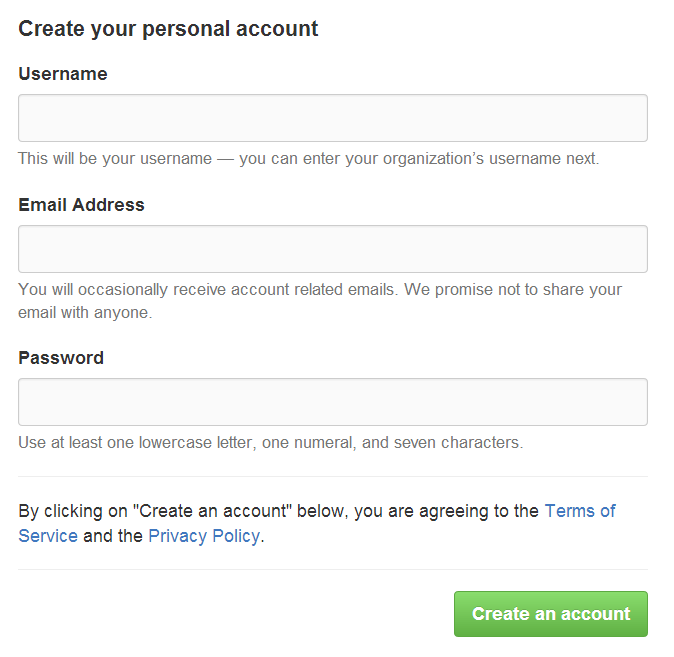
\includegraphics {fig/rejestracja}
	\caption{Formularz rejestracyjny repozytorium GitHub}
	\label{fig:rejestracja}
\end{figure}
Nastepnie z menu na górze po prawej stronie wybieramy opcję "New repository"
\begin{figure}
	\centering
	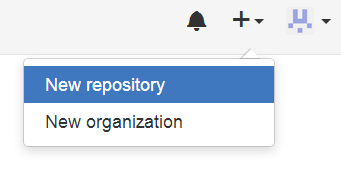
\includegraphics{fig/new_project}
	\caption{Tworzenie nowego repozytorium}
	\label{fig:new_project}
\end{figure}
Uzupełniamy dane dotyczące projektu. Musimy mu nadać nazwę, możemy opcjonalnie dodać opis tworzonego repozytorium, oraz zdecydować czy projekt będzie publiczny czy prywatny

\begin{figure}
	\centering
	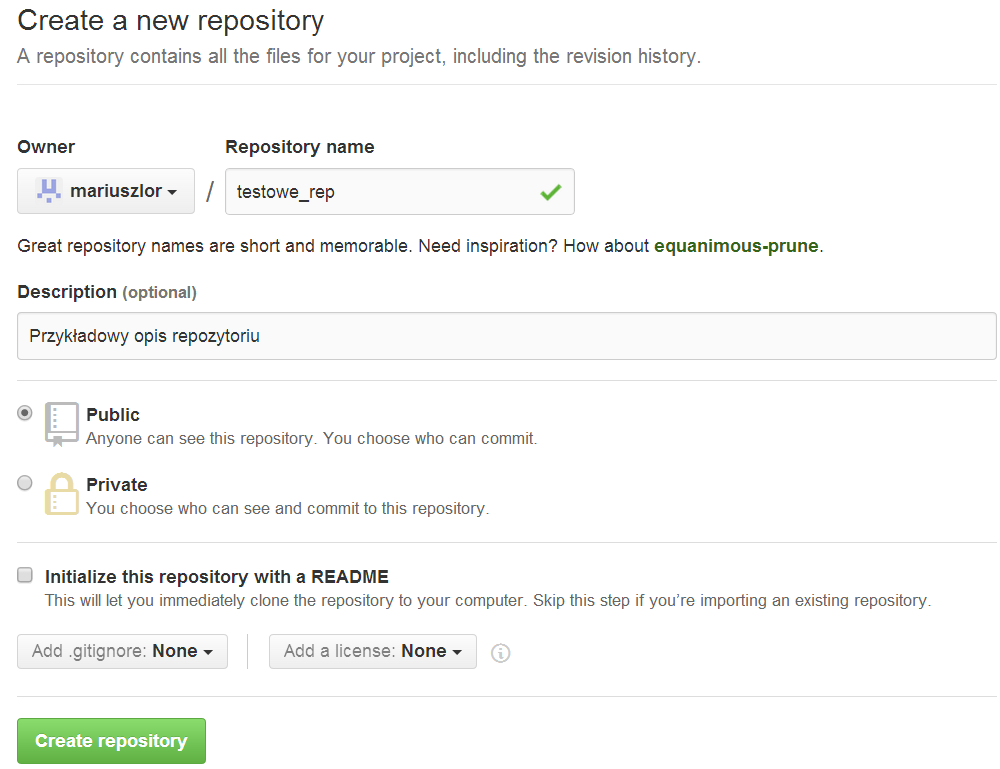
\includegraphics{fig/new_project_2}
	\caption{Uzupełniamy dane na temat projektu}
	\label{fig:new_project2}
\end{figure}
Teraz możemy dodać kolejnych uczestników projektu wybierając z menu opcję "New collaborator"
Uczestników możemy wyszukiwać  według róznych kryteriów
\begin{figure}
	\centering
	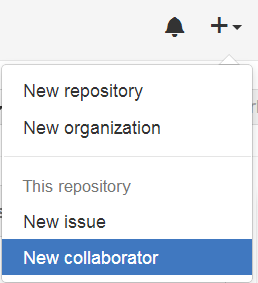
\includegraphics{fig/collaborator}
	\caption{Dodawanie nowego uczestnika projektu}
	\label{fig:collaborator}
\end{figure}
\begin{figure}
	\centering
	
\includegraphics{fig/add_collaborator}
	\caption{Mamy możliwość wyszukiwania nowych członków według różnych kryteriów}
	\label{fig:add_collaborator}
\end{figure}
Aby mieć możliwość wysyłania plików do repozytorium musimy zainstalować program na swoim systemie w tym celu wchodzimy na stronę \href{https://desktop.github.com/}{https://desktop.github.com/}.\\ Program możemy zainstalować w systemach:
\begin{enumerate}
\item Windows 7
\item Windows 8/8.1
\item Windows 10
\end{enumerate}
Starsze wersję systemów operacyjnych nie są wspierane\\
Dostępna jest również wersja dla komputerów MAC z systemem OS X 10.9 lub nowszym
\begin{figure}
	\centering
	
\includegraphics{fig/gitdownload}
	\caption{Przycisk umożliwiający pobranie programu}
	\label {fig:gitdownload} 
\end{figure}



% początkowy opis projektu
\chapter{Piotr Jabłoński}

%Piotr Jabłoński		
\chapter{Mirosława Pelc}

Mirosława Pelc
Swing to biblioteka graficzna używana w języku programowania Java. To właśnie z tej biblioteki skorzystałam tworząc interfejs graficzny. Tworzenie GUI rozpoczęłam od „bazy” czyli okna głównego, zwanego JFrame w środowisku programistycznym. W tym celu należało rozszerzyć klasę odpowiadającą za okno główne dodając słowo extends a zaraz po nim JFrame.
\begin{verbatim}
public class MainWindow extends JFrame \{
private static final long serialVersionUID = -4321522332774571523L;

public static void main (String[]args)\{
new MainWindow().setVisible(true);
\}

public MainWindow() \{
setMinimumSize(new Dimension(700, 500));
setDefaultCloseOperation(JFrame.DISPOSE\_ON\_CLOSE);
setLayout(new BorderLayout());

setJMenuBar(Tools.aboutMenu(new JMenuBar(), MainWindow.this));

try \{
InputStream imgIS = getClass().getResourceAsStream("/szachy.png");
add(new JLabel(new ImageIcon(ImageIO.read(imgIS))), BorderLayout.CENTER);
\} catch (IOException e1) \{
e1.printStackTrace();
\}
\}
\}
\end{verbatim}
W powyższym kodzie ustawiłam rozmiar okna komendą setMinimumSize, dodałam obrazek startowy używając InputStream oraz ImageIcon. Stworzyłam pasek menu używając takich komponentów jak JMenu, JMenuItem, MenuBar. Tworzenie paska menu:
\begin{verbatim}
JMenu 	mnTurniej 	 = new JMenu("Turniej"),
mnOProgramie = new JMenu("O programie");
menuBar.add(mnTurniej);
menuBar.add(mnOProgramie);

JMenuItem 	mntmPomoc 		= new JMenuItem("Pomoc"),
dodajTurniej 	= new JMenuItem("Dodaj turniej"),
wybierzTurniej	= new JMenuItem("Wybierz turniej"),
mntmAutorzy 	= new JMenuItem("Autorzy"),
mntmOpis 		= new JMenuItem("Opis");

mntmPomoc.setAlignmentY(Component.TOP\_ALIGNMENT);

mnTurniej.add(dodajTurniej);
mnTurniej.add(wybierzTurniej);
mnOProgramie.add(mntmPomoc);
mnOProgramie.add(mntmAutorzy);
mnOProgramie.add(mntmOpis);

dodajTurniej.setAccelerator(KeyStroke.getKeyStroke(
java.awt.event.KeyEvent.VK\_F2, 0));
wybierzTurniej.setAccelerator(KeyStroke.getKeyStroke(
java.awt.event.KeyEvent.VK\_F3, 0));

dodajTurniej.addActionListener(e -> \{
frame.getContentPane().removeAll();
frame.add(new AddTPanel(frame), BorderLayout.CENTER);
frame.pack();
\});
wybierzTurniej.addActionListener(e -> \{
frame.getContentPane().removeAll();
frame.add(new ShowTPanel(frame), BorderLayout.CENTER);
frame.pack();
\});
// otwieranie pdf z instrukcją po wybraniu pomocy
mntmPomoc.addActionListener(e->\{
if(Desktop.isDesktopSupported()) \{
try \{
File myFile = new File("turniej.pdf");
Desktop.getDesktop().open(myFile);
\} catch (IOException ex) \{
System.out.println(e);
\}
\}
\});
\end{verbatim}
Dodane zostały skróty klawiszowe dla poszczególnych JMenuItem. Okno po wykonaniu czynności wygląda następująco:
\begin{figure}[H]
	\centering
	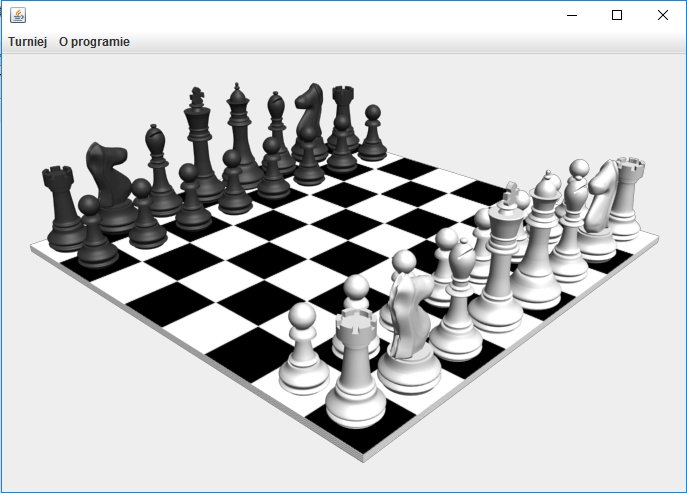
\includegraphics[width=10cm]{fig/m1}
	\caption{Skróty klawiszowe dla poszczególnych JMenuItem}
	\label {fig:JMenuItem} 
\end{figure}
Aby utworzyć nowy turniej potrzebnym było stworzenie nowego panelu, który łączy się z bazą danych. Oto jego kod:
\begin{verbatim}
package window;

import java.awt.Font;
import java.awt.event.ActionEvent;
import java.awt.event.ActionListener;
import java.util.Calendar;

import javax.swing.JButton;
import javax.swing.JFrame;
import javax.swing.JLabel;
import javax.swing.JPanel;
import javax.swing.JTextField;
import javax.swing.SwingConstants;

import model.Database;
import model.Tournament;
import panel.CompetitorTabbedPane;

/**
* Panel "nowy turniej"
*/
public class AddTPanel extends JPanel \{
private static final long serialVersionUID = -4930339429679727134L;
private JTextField textField;
private String nazwa;

public AddTPanel(final JFrame jframe)\{
setLayout(null);

JLabel nameTour = new JLabel("Nazwa turnieju");
nameTour.setFont(new Font("Consolas", Font.PLAIN, 16));
nameTour.setHorizontalTextPosition(SwingConstants.CENTER);
nameTour.setHorizontalAlignment(SwingConstants.CENTER);
nameTour.setBounds(100, 100, 484, 30);
add(nameTour);

textField = new JTextField();
textField.setBounds(100, 141, 484, 25);
textField.setColumns(10);
add(textField);

JButton addButton = new JButton("Utwórz");
addButton.setFont(new Font("Consolas", Font.PLAIN, 16));
addButton.setBounds(100, 293, 484, 30);
addButton.addActionListener(new ActionListener() \{
public void actionPerformed(ActionEvent e) \{
nazwa=textField.getText();
String year = String.valueOf(Calendar.getInstance().get(Calendar.YEAR));
Tournament t = new Tournament(null,nazwa,year,8,5,-1);
Database db = new Database();
db.insertOrUpdateTournament(t);
jframe.getContentPane().removeAll();
new CompetitorTabbedPane(t, jframe);
db.close();
\}
\});

// po naciśnięciu enter aktywuje się guzik DODAJ
jframe.getRootPane().setDefaultButton(addButton);

add(addButton);
\}
\}
\end{verbatim}
Panel zawiera takie komponenty jak JPanel, etykietę JLabel, pole tekstowe JTextField oraz guzik JButton. Stworzony panel wygląda następująco:
\begin{figure}[H]
	\centering
	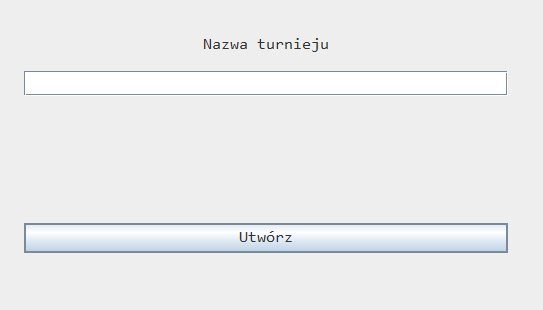
\includegraphics[width=10cm]{fig/m2}
	\caption{Komponenty panelu}
	\label {fig:panel} 
\end{figure}

Kolejnym krokiem było utworzenie panelu, który odpowiadałby za wybór wcześniej utworzonego turnieju. Kod tego panelu przedstawia się następująco:
\begin{verbatim}
package window;

import java.awt.Font;
import java.awt.event.ActionEvent;
import java.awt.event.ActionListener;

import javax.swing.JComboBox;
import javax.swing.JFrame;
import javax.swing.JLabel;
import javax.swing.JPanel;
import javax.swing.SwingConstants;

import model.Database;
import model.Tournament;
import panel.CompetitorTabbedPane;

/**
* Panel "dodaj turniej"
*/
public class ShowTPanel extends JPanel \{
private static final long serialVersionUID = -1094699102373510646L;
private Database db;

public ShowTPanel(final JFrame jframe) \{
db = new Database();
setLayout(null);

final JComboBox<String> comboBox = new JComboBox<String>();
comboBox.setFont(new Font("Consolas", Font.PLAIN, 15));
comboBox.setBounds(10, 100, 664, 30);

for(Tournament t: db.getTournaments())\{
String nazwa = t.getName();
comboBox.addItem(nazwa);
\}

comboBox.addActionListener (new ActionListener () \{
public void actionPerformed(ActionEvent e) \{
int sIndex = comboBox.getSelectedIndex();
jframe.getContentPane().removeAll();
new CompetitorTabbedPane(db.getTournaments().get(sIndex),jframe);
db.close();
\}
\});

add(comboBox);

JLabel wybierz = new JLabel("Wybierz turniej");
wybierz.setFont(new Font("Consolas", Font.PLAIN, 16));
wybierz.setHorizontalTextPosition(SwingConstants.CENTER);
wybierz.setHorizontalAlignment(SwingConstants.CENTER);
wybierz.setBounds(10, 59, 664, 30);
add(wybierz);		
\}	
\}
\end{verbatim}
Użyte komponenty to w tym przypadku etykieta JLabel oraz JComboBox czyli wysuwana lista, która zawiera nazwy zapisanych turniejów. Oto graficzna reprezentacja panelu wyboru turnieju:
\begin{figure}[H]
	\centering
	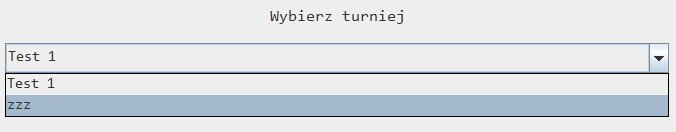
\includegraphics[width=10cm]{fig/m3}
	\caption{Graficzna reprezentacja panelu wyboru turnieju}
	\label {fig:G} 
\end{figure}

Po zatwierdzeniu utworzonego turnieju lub po wybraniu już istniejącego pojawia się okno odpowiadające za rozgrywki. Początkowo są trzy zakładki, których kod jest następujący:
\begin{verbatim}
public CompetitorTabbedPane(Tournament turniej, JFrame frame)\{
this.turniej = turniej;
this.DB = new Database();
showPanel = new ShowEditCompetitorPanel(turniej, DB);
tournamentPanel = new TournamentPanel(turniej, DB);
[…]
groupsPanel = new GroupsPanel(turniej, DB, tStartlistener);
setMenu(frame);
tabbedPane.add(Strings.showOrEditComp, showPanel);
tabbedPane.add(Strings.tournament, tournamentPanel);
tabbedPane.add(Strings.prepGroups, groupsPanel);
tabbedPane.addChangeListener((e) -> \{
int i = tabbedPane.getSelectedIndex();
if(i==0) showPanel.setData();
if(i==1) tournamentPanel.setSBBounds();
if(i==2) groupsPanel.initComponents();
if(i==3) gamesPanel.initComponents();
if(i==5) finaleGamesPanel.initComponents();
comp.setVisible( turniej.isPlayersEditAllowed() \&\& i==0);
group.setVisible(turniej.isPlayersEditAllowed() \&\& i==2 );
sort.setVisible(i==2);
\});

frame.add(tabbedPane);
setVisible(true);
\end{verbatim}
Użyty został komponent JTabbedPane, który odpowiada za panel z zakładkami. 

Jak można łatwo zauważyć, program ma wiele tabelek. JTable to kolejny komponent biblioteki Swing. Przykładowe tabele:
\begin{verbatim}
private JTable table;
[…]
table = new EditCompetitorJTable();
[…]
public class EditCompetitorJTable extends JTable \{
private static final long serialVersionUID = -9074329149984999956L;

public EditCompetitorJTable() \{
super();
setIntercellSpacing(new Dimension(25, 2));
setRowHeight(20);
setModel(new EditCompetitorTableModel());

setSelectionMode(javax.swing.ListSelectionModel.SINGLE\_SELECTION); 
// pole tekstowe akceptujące tylko znaki a-Z, - i spację
final JTextField jtf = new JTextField(new MyPlainDocument(), null, 0);
// przy rozpoczęciu edyji zaznaczenie wszystkiego
jtf.addFocusListener(new FocusAdapter() \{
@Override
public void focusGained(FocusEvent e) \{
jtf.selectAll();
\}
\});

// dla pól imię i nazwisko ustawiony edytor na podstawie powyższego pola tekstowego 
columnModel.getColumn(1).setCellEditor(new DefaultCellEditor(jtf));
columnModel.getColumn(2).setCellEditor(new DefaultCellEditor(jtf));
columnModel.getColumn(4).setCellEditor(new DefaultCellEditor(
new JComboBox<Integer>(new Integer[]\{1,2,3,4,5,6\})
));
\}

// po przejśiu do komórki (również tabulatorem) rozpoczęcie edycji
public void changeSelection(int row, int column, boolean toggle, boolean extend) \{
super.changeSelection(row, column, toggle, extend);
if(editCellAt(row, column)) \{
getEditorComponent().requestFocusInWindow();
\}
\}
\}
\end{verbatim}
\begin{verbatim}
JTable table = new JTable(new MyTableModel());
table.getColumnModel().getColumn(3).setCellEditor(new DefaultCellEditor(
new JComboBox<String>(new String[] \{Strings.notPlayedYet, Strings.whiteWon, Strings.blackWon, Strings.tie\})
));
table.setDefaultRenderer(String.class, new MyCellRenderer());
add(new JScrollPane(table));
\end{verbatim}
A oto kod odpowiadający za formatowanie JTable
\begin{verbatim}
public class EditCompetitorJTable extends JTable \{
private static final long serialVersionUID = -9074329149984999956L;

public EditCompetitorJTable() \{
super();
setIntercellSpacing(new Dimension(25, 2));
setRowHeight(20);
setModel(new EditCompetitorTableModel());

setSelectionMode(javax.swing.ListSelectionModel.SINGLE\_SELECTION); 
// pole tekstowe akceptujące tylko znaki a-Z, - i spację
final JTextField jtf = new JTextField(new MyPlainDocument(), null, 0);
// przy rozpoczęciu edyji zaznaczenie wszystkiego
jtf.addFocusListener(new FocusAdapter() \{
@Override
public void focusGained(FocusEvent e) \{
jtf.selectAll();
\}
\});

// dla pól imię i nazwisko ustawiony edytor na podstawie powyższego pola tekstowego 
columnModel.getColumn(1).setCellEditor(new DefaultCellEditor(jtf));
columnModel.getColumn(2).setCellEditor(new DefaultCellEditor(jtf));
columnModel.getColumn(4).setCellEditor(new DefaultCellEditor(
new JComboBox<Integer>(new Integer[]\{1,2,3,4,5,6\})
));
\}

// po przejśiu do komórki (również tabulatorem) rozpoczęcie edycji
public void changeSelection(int row, int column, boolean toggle, boolean extend) \{
super.changeSelection(row, column, toggle, extend);
if(editCellAt(row, column)) \{
getEditorComponent().requestFocusInWindow();
\}
\}
\}
\end{verbatim}

Aby nie powielać kodu przy formatowaniu modelu JTable stworzyłam klasę abstrakcyjną modelu rozszerzającą AbstractTableModel, którą przypisuję do tabeli.
\begin{verbatim}
protected abstract class MyTableModel extends AbstractTableModel \{
private static final long serialVersionUID = -8079013606990307646L;
final String[] columnNames = \{Strings.board, Strings.playsWithWhite, Strings.playsWithBlack, Strings.score\};
@Override
public Class<?> getColumnClass(int columnIndex) \{
return String.class;
\}
@Override
public int getColumnCount() \{
return 4;
\}
@Override
public String getColumnName(int columnIndex) \{
return columnNames[columnIndex];
\}
@Override
public int getRowCount() \{
return singleGames.size();
\}
@Override
public Object getValueAt(int row, int col) \{
SingleGame sg = singleGames.get(row);
if(col==0 \&\& sg.getBoard()==-1) return " - ";
if(col==0) return sg.getBoard()+1;
if(col==1) return competitorMap.get(sg.getCompetitorW());
if(col==2) return competitorMap.get(sg.getCompetitorB());
if(col==3) \{
if(sg.getScore()==0) return Strings.notPlayedYet;
if(sg.getScore()==1) return Strings.whiteWon;
if(sg.getScore()==2) return Strings.blackWon;
if(sg.getScore()==3) return Strings.tie;
\}
return null;
\}
public abstract void setValueAt(Object aValue, int row, int col);
\}
\}
\end{verbatim}

W celu ułatwienia użytkownikowi programu przydzielanie zawodników do szachownic, komórki  JTable zostały pokolorowane. Oto jak wygląda to w kodzie programu:
\begin{verbatim}
final void recalcColors() \{
currentlyPlayedGames = new ArrayList<>(turniej.getBoards());
currentlyPlayedGames.clear();;
List<Integer> 	playingCompetitors 	= new ArrayList<>(2*turniej.getBoards()),
freeBoards 			= new LinkedList<>();
for(int i=0; i<turniej.getBoards(); ++i) freeBoards.add(i);
for(SingleGame sg : singleGames.stream().filter(g->g.getScore()==0\&\&g.getBoard()>=0)
.collect(Collectors.toList()))\{
freeBoards.remove(sg.getBoard());
playingCompetitors.add(sg.getCompetitorW());
playingCompetitors.add(sg.getCompetitorB());
currentlyPlayedGames.add(sg);
\};
for(SingleGame sg : singleGames.stream().filter(g->g.getScore()==0\&\&g.getBoard()<0)
.collect(Collectors.toList()))\{
if(freeBoards.isEmpty()) break;
if(!playingCompetitors.contains(sg.getCompetitorW()) \&\&
!playingCompetitors.contains(sg.getCompetitorB())) 
\{
int board = freeBoards.get(0);
sg.setBoard(board);
freeBoards.remove(0);
playingCompetitors.add(sg.getCompetitorW());
playingCompetitors.add(sg.getCompetitorB());
currentlyPlayedGames.add(sg);
\}	
\};
sortGames();
\}
\end{verbatim}
\begin{verbatim}
package res;

import java.awt.Color;

public final class Colors \{
public final static Color 
selInProgress 	= Color.decode("\#5BFFB5"),
selNormal		= Color.decode("\#84D4FF"),
InProgress		= Color.decode("\#5BFF8C"),
normal 			= Color.decode("\#FFFFFF");
\}
\end{verbatim}

Druga zakładka w oknie turnieju to edycja turnieju, czyli: zmiana tytułu, ustawienie roku rozgrywania turnieju, suwaki odpowiedzialne za ilość szachownic, czas rozgrywki, ilość grup. Użyte komponenty to etykieta JLabel, pole tekstowe JTextField, suwak ScrollBar. Layout panelu ustawiony jest na GridLayout(0,2,…) co oznacza, że panel podzielony jest na dwie kolumny a komponenty dodawane są raz do jednej kolumny, raz do drugiej. Oto kod TournamentPanel:
\begin{verbatim}
package panel;

import java.awt.BorderLayout;
import java.awt.Component;
import java.awt.GridLayout;
import java.awt.Scrollbar;

import javax.swing.JLabel;
import javax.swing.JPanel;
import javax.swing.JTextField;
import javax.swing.border.EmptyBorder;
import javax.swing.event.DocumentEvent;
import javax.swing.event.DocumentListener;

import model.Database;
import model.Tournament;
import res.Strings;
import tools.MyPlainDocument;
import tools.Simulator;

/**
* Zakładka danych o turnieju
*/
public class TournamentPanel extends JPanel\{
private static final long serialVersionUID = -3657045958131642437L;
private final Tournament turniej;
private final Database DB;
private final JLabel nameL, yearL, sgTimeL, groupsL, boardsL, stats1L, stats2L;
final JTextField nameTF, yearTF;
final Scrollbar groupsSB, sgTimeSB, boardsSB;
final JPanel panel = new JPanel();
/**
* @param t - id turnieju
* @param db - baza danych
*/
public TournamentPanel(Tournament t, Database db)\{
this.turniej = t;
this.DB = db;
nameL 	= new JLabel("Nazwa turnieju: ");
yearL 	= new JLabel("Rok: ");
sgTimeL = new JLabel(Strings.sgTimeT+"10 min");
groupsL = new JLabel(Strings.groupsT+"2");
boardsL = new JLabel(Strings.boardsT);
stats1L = new JLabel(Strings.gamesT);
stats2L = new JLabel(Strings.timeRRET);
nameTF 	= new JTextField();
yearTF  = new JTextField();
groupsSB 	= new Scrollbar(Scrollbar.HORIZONTAL, 2, 1, 2, 9+1);
sgTimeSB 	= new Scrollbar(Scrollbar.HORIZONTAL, 20, 4, 2, 40+4);
boardsSB 	= new Scrollbar(Scrollbar.HORIZONTAL, 8, 1, 2, 20+1);

setLayout(new BorderLayout());
setBorder(new EmptyBorder(10, 10, 10, 10));
panel.setLayout(new GridLayout(0, 2, 10, 20));
add(panel, BorderLayout.NORTH);
nameTF.setDocument(new MyPlainDocument());
yearTF.setDocument(new MyPlainDocument());

setComponentsActions();

Component[] cs = \{
nameL, nameTF, yearL, yearTF, sgTimeL, sgTimeSB, groupsL, groupsSB, boardsL, boardsSB, stats1L, stats2L
\};
for(Component c : cs) panel.add(c);

nameTF.setText(turniej.getName());
yearTF.setText(turniej.getYear());
setSBBounds();
recalcStats();
\}

private void setComponentsActions() \{
nameTF.getDocument().addDocumentListener(new MyDocumentListener() \{			
@Override
public void action() \{
turniej.setName(nameTF.getText());
DB.insertOrUpdateTournament(turniej);
\}
\});
yearTF.getDocument().addDocumentListener(new MyDocumentListener() \{
@Override
public void action() \{
turniej.setYear(yearTF.getText());
DB.insertOrUpdateTournament(turniej);
\}
\});
groupsSB.addAdjustmentListener(e -> \{
if(!turniej.isPlayersEditAllowed()) \{
groupsSB.setValue(turniej.getRounds());
return;
\}
int g = groupsSB.getValue();
turniej.setRounds(g);
DB.insertOrUpdateTournament(turniej);
recalcStats();
\});
boardsSB.addAdjustmentListener(e -> \{
if(!turniej.isPlayersEditAllowed()) \{
boardsSB.setValue(turniej.getBoards());
return;
\}
int g = boardsSB.getValue();
turniej.setBoards(g);
DB.insertOrUpdateTournament(turniej);
recalcStats();
\});
sgTimeSB.addAdjustmentListener(e -> \{
recalcStats();
\});
\}

private abstract class MyDocumentListener implements DocumentListener \{
public abstract void action();
@Override public final void removeUpdate(DocumentEvent e) \{ action(); \}
@Override public final void insertUpdate(DocumentEvent e) \{ action(); \}
@Override public final void changedUpdate(DocumentEvent e)\{ action(); \}
\}

public void recalcStats() \{ // TODO - poprawić przewidywany czas turnieju
groupsL.setText(Strings.groupsT+groupsSB.getValue());
boardsL.setText(Strings.boardsT+boardsSB.getValue());
sgTimeL.setText(Strings.sgTimeT+(sgTimeSB.getValue()/2f)+" min");
int graczy = DB.getCompetitors(turniej.getId()).size();
if(turniej.getBoards()<1 || graczy<2) return;
float czasSG = sgTimeSB.getValue()/2f;
int grup = groupsSB.getValue();
int rozgrywek = Simulator.rozgrywek\_eliminacje(graczy, grup);
stats1L.setText(Strings.gamesT+String.valueOf(rozgrywek));
int gier\_naraz = (int)Math.min(Math.floor(graczy/2), turniej.getBoards());
stats2L.setText(Strings.timeRRET+Math.ceil(rozgrywek/gier\_naraz)*czasSG+" min");
\}
public void setSBBounds() \{
int graczy = DB.getCompetitors(turniej.getId()).size();
groupsSB.setMinimum(2);
groupsSB.setMaximum((int)Math.ceil(graczy/2)+2);
groupsSB.setValue(turniej.getRounds());
recalcStats();
\}
\}
\end{verbatim}
Poniższy rysunek przedstawia kod po skompilowaniu: 
\begin{figure}[H]
	\centering
	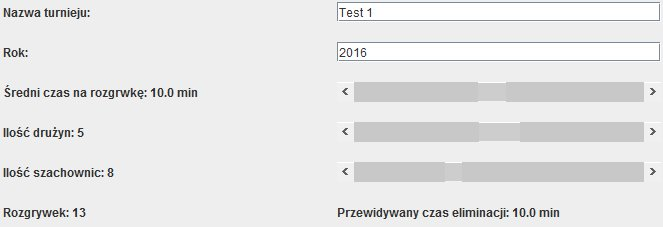
\includegraphics[width=10cm]{fig/m4}
	\caption{Edycja turnieju}
	\label {fig:EdycjaTurnieju} 
\end{figure}

Program nie dopuszcza do zaistnienia pewnych zdarzeń, jeśli użytkownik wprowadzi błędne dane lub dobierze zawodników źle w grupy wówczas wyskoczy błąd. Za wiadomości o błędach odpowiada JOptionPane. Na potrzemy programu stworzyłam kilka wiadomości o błędach. Kod:
\begin{verbatim}
package tools;

import javax.swing.JOptionPane;

import model.Competitor;

/**
* Definiuje okna błędów, ostrzeżeń oraz informacji
*/
public class Dialogs \{
public static void bladBazy() \{
JOptionPane.showMessageDialog(
null, 
"Błąd odczytu / zapisu", 
"Błąd bazy", 
JOptionPane.ERROR\_MESSAGE);
\}

public static void graczBezGrupy() \{
JOptionPane.showMessageDialog(
null, 
"Aby móc rozpocząć turniej, każdy gracz musi być przydzielony do grupy", 
"Gracz bez grupy", 
JOptionPane.ERROR\_MESSAGE);
\}

public static void nierownomiernyPodzial(int min, int max) \{
JOptionPane.showMessageDialog(
null, 
"Największa grupa: "+max+" uczestników, \textbackslash\{\}n"+
"Najmniejsza grupa: "+min+" uczestników \textbackslash\{\}n"+
"Różnica pomiędzy tymi wartościami nie może być większa od 1", 
"Nierównomierny podział", 
JOptionPane.ERROR\_MESSAGE);
\}

public static void gryBezWyniku() \{
JOptionPane.showMessageDialog(
null, 
"Aby zakończyć eliminacje, wszystkie gry tej fazy muszą być ukończone", 
"Nieukończone rozgrywki", 
JOptionPane.ERROR\_MESSAGE);
\}

public static void autorzy() \{
JOptionPane.showMessageDialog(
null,
"Autorzy: \textbackslash\{\}n"+
"Piotr Jabłoński\textbackslash\{\}n"+
"Mirosława Pelc\textbackslash\{\}n"+
"Mariusz Lorek",
"Autorzy", JOptionPane.UNDEFINED\_CONDITION);
\}

public static void opis() \{
JOptionPane.showMessageDialog(
null,
"Program powstał w ramach zaliczenia Zespołowych Przedsięwzięć Inżynierskich"+
"na Państwowej Wyższej Szkole Zawodowej w Nowym Sączu.\textbackslash\{\}nProwadzący przedmiot: "+
"dr Antoni Ligęza\textbackslash\{\}nProgram obsługuje turniej szachowy odbywający się podczas "+
"Małopolskiej Nocy Naukowców.",
"Opis", JOptionPane.UNDEFINED\_CONDITION);
\}

/**
* @return Czy kontynuować mimo ostrzeżenia
*/
public static boolean niktZGrupyDoFinalow() \{
int r = JOptionPane.showConfirmDialog(
null, 
"Istnieje grupa, w której nie wybrano graczy przechodzących do finału. Kontynuować?",
"Uwaga!",
JOptionPane.OK\_CANCEL\_OPTION);
return r==JOptionPane.OK\_OPTION;
\}

/**
* @return Czy na pewno zdyskwalifikowac
*/
public static boolean czyZdyskwalifikowac(Competitor c) \{
int r = JOptionPane.showConfirmDialog(
null, 
"Czy jesteś pewien, że chcesz zdywkwalifikować zawodnika "+c+"?\textbackslash\{\}nTej operacji nie można cofnąć",
"Uwaga!",
JOptionPane.OK\_CANCEL\_OPTION);
return r==JOptionPane.OK\_OPTION;
\}
\}
\end{verbatim}
Tak wygląda przykładowe okno informujące o błędzie:
\begin{figure}[H]
	\centering
	
\includegraphics[width=10cm]{fig/m5}
	\caption{Okno informujące o błędzie}
	\label {fig:OknoBledu} 
\end{figure}

Podczas generowania losowych graczy imiona i nazwiska pobierane są z plików imiona.txt oraz nazwiska.txt, które zawarte są w pliku jar. Poniżej pokazałam jak to się odbywa w programie:
\begin{verbatim}
public static Competitor RandomPlayer() throws IOException \{
Random rn = new Random();
int a = 10+rn.nextInt(10)+rn.nextInt(10);
int c = rn.nextInt(6)+1;

int randomInt = rn.nextInt(300);
String imie = null, nazwisko = null;

InputStream imionaIS = JFrame.class.getResourceAsStream("/imiona.txt");
InputStream nazwiskaIS = JFrame.class.getResourceAsStream("/nazwiska.txt");

imieReader = new BufferedReader(new InputStreamReader(imionaIS, "UTF-8"));
nazwiskoReader = new BufferedReader(new InputStreamReader(nazwiskaIS, "UTF-8"));

imieReader.mark(0);
nazwiskoReader.mark(0);

do \{
imieReader.reset();
nazwiskoReader.reset();
for (int i = 0; i < randomInt; i++) \{
imie = imieReader.readLine();
nazwisko = nazwiskoReader.readLine();
\}
\} while(imie==null || nazwisko==null || (imie.endsWith("a") \&\& nazwisko.endsWith("ki")));
return new Competitor(null, imie, nazwisko, a, c, false, null);
\}
\end{verbatim}

%Mirosława Pelc
\chapter{Mariusz Lorek}
%Mariusz Lorek
%Usuwa numeracje z naglowka. Zapewnia  dodanie do spisu tresci
\setcounter{secnumdepth}{-1}


%Gdy mamy dużą bibliografię to możemy wybierać pozycje,
%które cytujemy
%\nocite{ad-tg-80}

%Dodaje wszystkie pozycje z bibliografii
%\nocite{*}

%Po kazdym dodaniu nowej pozycji bibliograficznej
%z katalogu glownego uruchom: bibtex pracadyp
%\bibliographystyle{pdplain}
%\bibliography{tex/pracadyp}

\begin {thebibliography}{11}
\bibitem{Balcerzak2005} Balcerzak J., Pansiuk J.: \emph{Wprowadzenie do kartografii matematycznej}, Warszawa, OWPW~2005.
\bibitem{Barrett} Barrett R. i inni: \emph{Templates for the Solution of Linear Systems: Building Blocks for Iterative Methods1}, wersja elektorniczna Mathematics http://www.siam.org/books.
\bibitem{bjork} Bjork A., Dahlquist G.: \emph{Numerical Methods in Scientific Computing}, Philadelphia, SIAM~2002.
\bibitem{CCITTG4}CCITT, \emph{Facsimile Coding Schemes and Coding Control Functions for Group 4 Facsimile
Apparatus, Recommendation T.6, Volume VII, Fascicle VII.3, Terminal Equipment and
Protocols for Telematic Services, The International Telegraph and Telephone Consultative Committee (CCITT)}, Geneva, CCITT~1985.
\bibitem{drwal:mathematica2000} Drwal G, i in., \emph{Mathematica 4}, Gliwice, WPKJS~200.
\bibitem{Gdowski1982} Gdowski B.: \emph{Elementy geometrii rózniczkowej w zadaniach}, Warszawa, PWN~1982.
\bibitem{Gotlib2007} Gotlib D., Iwaniak A., Olszewski R.: \emph{GIS obszary zastosowań}, Warszawa, PWN~2007.
\bibitem{INTERGRAPHFileFormat1994} INTERGRAPH: \emph{INTERGRAPH RASTER FILE FORMAT REFERENCE GUIDE}, Alabama, Intergraph Corporation~1994.
\bibitem{Januszewski2006} Januszewski J.: \emph{Systemy satelitarne GPS, Galileo i inne}, Warszawa, PWN~2006.
\bibitem{kielbasinski1992}: Kiełbasiński A., Schwetlick H.: \emph{Numeryczna algebra liniowa}, Warszawa, WNT~1992.
\bibitem{Kincaid2006} Kincaid D.: \emph{Analiza numeryczna}, Warszawa, WNT~2006.
\bibitem{Lamparski2001}Lamparski J.: \emph{Navstar GPS od teorii do praktyki}, Olsztyn, WUW-M~2001.
\bibitem{Levine1994} Levine J.: \emph{Programowanie plików graficznych w C/C++}, New York, Wiley~1994.
\bibitem{Longley2006} Longley P. i inni: \emph{GIS teoria i praktyka}, Warszawa, PWN~2006.
\bibitem{GML:opengis} Open Geospatial Consortium Inc.: \emph{OpenGIS Geography Markup Language (GML) Encoding Standard, Version: 3.2.1},  OGC~2007.
\bibitem{GML:opengisimplemntation} Open Geospatial Consortium Inc.: \emph{OpenGIS® Geography Markup Language (GML) Implementation Specification}, OGC~2004.
\bibitem{Opera2002} Opera J.: \emph{Geometria róniczkowa i jej zastosowania}, Warszawa, PWN~2002.
\bibitem{Poczobut1982Geogeza} Odlanicki-Poczobut M.: \emph{Geodezja}, PPWK~1982.
\bibitem{Li2007}Li Y. i inni: \emph{GML Topology Data Storage Schema Design}, Chiba University~2007.
\bibitem{li2004GMLstorage}Li Y., Li J., Zhou S.: \emph{GML Storage}, A Spatial Database Approach,ER (Workshops), str 55-66, 2004.
\bibitem{Sayood2002} Sayood K.: \emph{Kompresja danych}, Warszawa, Rm~2002.
\bibitem{G52003} \emph{The Technical Instruction G-5, The Ground Cadastre and Buildings, The Main Surveying and
Cartographic Bureau}, Warszawa 2003.



\end {thebibliography}


\listoffigures

%\listoftables %Każdy członek zespołu musi dołożyć minimum 5 pozycji bibliograficzny, które posłużyły mu do opracowania zadanego fragmentu projektu.
\end{document}

To robi tylko kierownik projektu:
Wprowadź polecenie ze swoimi danymi
svn co https://riouxsvn.com/svn/zpi2014 --username aligeza

w bieżącym katalogu zostanie utworzony katalog z nazwą repozytorium, u mnie zpi2014

Skopiuj do niego całą zawartość projektu do katalogu zpi2014
przejdź do niego i wprowadź
svn add * --force
to polecenie dodało wszystkie pliki i podkatalogu do lokalnej kopii repozytorium.


Poniższe polecenie wyśle dane na serwer svn
svn commit -m "inicjacja dokumentacji projektu"


Teraz każdy członek z zespołu wykonuje polecnie ze swoim loginem!!!!!!!
Wprowadź polecenie ze swoimi danymi
svn co https://riouxsvn.com/svn/zpi2014 --username aligeza
Już każdy posiada swoje repozytorium do kompilacji.
Zmiany nanosić w swoim pliku i po porawnej kompilacji
trzeba przesłać na serwer z adekwatnym komentarzem
svn commit -m "Model stanowiska do zobrazowań"